\section{白炽电灯}\label{sec:11-2}

白炽电灯是最普通的电灯,它是利用电流热效应制成的。
当电流通过灯丝时,灯丝热到白炽状态\footnotemark 就发出很亮的光,可以供我们照明。
\footnotetext{物体温度达到 1700 ℃ 以上就发白光,这种状态叫白炽状态。}

白炽电灯的灯丝是用熔点高的钨做的,发光时温度在 2000 ℃ 以上。
为了防止钨在高温下氧化,小功率的灯泡都抽成真空,60 瓦特以上的灯泡充入氮、氩等气体。
充气灯泡里的气体可以阻碍钨丝在高温下的升华,灯丝温度可以提高到 2400 ~ 2700 ℃ ,
灯丝温度越高,消耗的电能中转化为光能的越多。

常用的白炽灯泡有螺丝口和卡口两种。
螺丝口灯泡的灯丝两头各焊接一根金属丝,这两根金属丝分别焊在灯泡尾部中心的金属块和螺旋上。
照明电路的两条导线,一条接在灯座里金属片上,一条接在灯座的螺旋套上(图 \ref{fig:11-2})。
把灯泡拧进灯座,灯泡尾部的金属块跟灯座里的金属片接触,灯泡尾部的螺旋跟灯座的螺旋套接触。
这样,灯丝就跟电路连通了。

\begin{figure}[htbp]
    \centering
    \begin{minipage}{7cm}
    \centering
    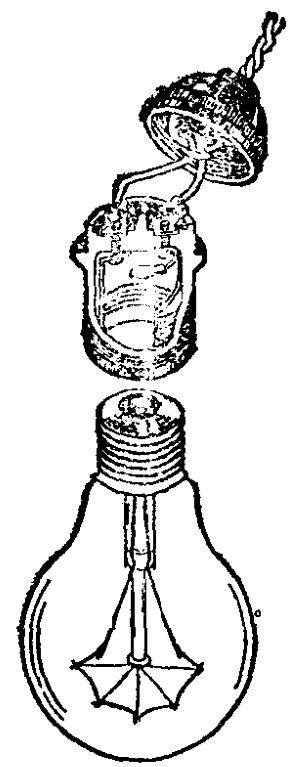
\includegraphics[width=4cm]{../pic/czwl2-ch11-2}
    \caption{螺丝口灯泡和灯座}\label{fig:11-2}
    \end{minipage}
    \qquad
    \begin{minipage}{7cm}
    \centering
    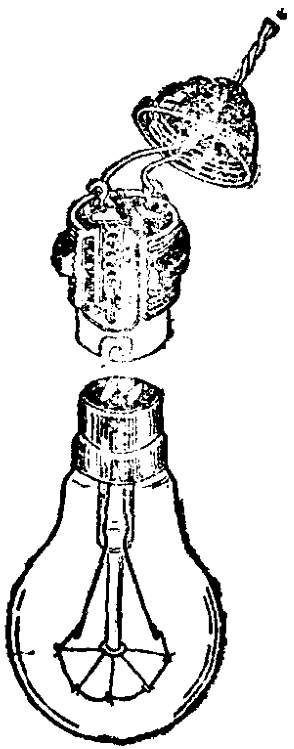
\includegraphics[width=4cm]{../pic/czwl2-ch11-3}
    \caption{卡口灯泡和灯座}\label{fig:11-3}
    \end{minipage}
\end{figure}

卡口灯泡中焊接在灯丝两头的两根金属丝,都从灯泡尾部伸出,分别用锡焊住(图 \ref{fig:11-3})。
灯座里有两根带弹簧的金属柱,分别跟照明电路的两条导线连接。
把灯泡插入灯座,并向顺时针方向稍稍旋转,灯泡就卡在灯座里,这时灯泡末端的两点焊锡分别跟两个金属柱接触。
这样,灯丝就跟电路连通了。


\section*{阅读材料:爱迪生和白炽电灯}

大家都说白炽电灯是爱迪生发明的。其实他并不是最先制成白炽电灯的人,
但是他最先制成实用、经济的白炽电灯,而且建成能给分散在千家万户的电灯供电的电力系统。
他的贡献的意义,不仅仅是照明史上的一次划时代的变革,而且为电能在其他方面的应用准备了条件,
对电力工业的发展起了巨大的推动作用。

爱迪生决心解决白炽电灯问题是在 1878 年 9 月。在这以前的五十多年里已经有许多人研制白炽电灯了。
最初是用铂作灯丝。铂是化学性质最稳定的元素,即使在高温时也很难跟其他元素化合,但是熔点只有 1772 ℃ ,
刚达到白炽状态再继续通电就烧断了。从 1840 年前后开始,人们改用熔点超过 3500 ℃ 的碳作灯丝。
碳很容易氧化,必须装在抽去空气的玻璃泡里。由于抽气技术水平低,泡内残存着大量氧分子,
高温时跟碳化合,所以碳丝亮不了几分钟就烧断了。

因此,爱迪生研制白炽电灯必须解决灯丝的材料问题。但是,最初爱迪生着重考虑的问题是,
必须具备什么条件,才可以使将来发明的白炽电灯能实际用来给千家万户照明,而不是只供少数人观赏。
他从当时的煤气灯系统得到启发,想到应该有个相当于中心煤气站的中心发电站,给各户供应廉价的电。
所有的白炽电灯都应并联着,以便用户可以随意开关电路中的每一盏灯。
非常重视研制成果的实际应用和经济效益,是爱迪生的突出特点。

最初爱迪生选用碳作灯丝材料,因为碳的熔点最高。
他把碳化的纸条\footnote{碳化是把材料放在密闭的坩锅内加热,使材料变成碳。}
放在抽出空气的玻璃泡里,维持白炽状态达 8 分钟。
以后改用耐高温的金属,试用了铂、铱、钼、锇等熔点高的金属,也想到过钨,但当时没有加工工具。
经过多次失败以后,他又回到了碳,试验什么材料碳化后作灯丝最好。
同时他努力改进抽气机和发电机,把灯泡里残余空气的压强从几万分之一大气压减小到百万分之一大气压,
把发电机的效率从 $40\%$ (这在当时是最高的)提高到 $90\%$。
据说他先后试验了一千六百多种材料,到 1879 年 10 月 21 日制成由碳化棉作灯丝的高真空白炽灯泡,寿命达 13.5 小时。
后来他又改用碳化的竹子纤维作灯丝,把灯泡寿命长到上千小时。
1882 年爱迪生在纽约建立了第一个中心发电站,开创了电照明的新时代。

在研制白炽电灯的过程中,爱迪生和他的助手们常常连续几天日夜不停地试验,吃、睡在实验室中。
这位只上过三个月小学、全靠自学成才的大发明家,除了亲自动手试验,还夜以继日地阅读科学书刊和学术论文。
有一次,他的朋友当面称赞他是天才,他笑了笑说:“天才,不过是百分之一的灵感加上百分之九十九的汗水!”



\lianxi

(1) 观察你所在的教室(或者你家里)的照明设备,总共有几个插座、几盏电灯、几个开关,
每个开关各控制几盏电灯,这些插座、电灯、开关是怎样连接着的?画出电路图。

(2) 找一个卡口灯泡,观察灯丝两端各连在尾部的什么地方。
找一个灯座,观察它的构造,看看它是怎样把电灯泡接入照明电路的。

(3) 找两个额定电压相同而额定功率不同的白炽电灯,例如一个是 “220V \; 15W” ,另一个是 “220V \; 100W”。
仔细观察哪个的灯丝比较细,想想看,哪个的灯丝电阻大?哪个灯泡比较亮?为什么?

注意:白炽电灯的灯丝一般是绕成螺旋形(图 \ref{fig:11-4}),以减少散热,提高灯丝温度。
因而观察时可能把螺旋的直径误认为是灯丝的直径。但是灯丝越细,绕成的螺旋也越细。

\begin{figure}[H]%[htbp]
    \centering
    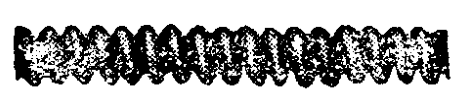
\includegraphics[width=0.4\textwidth]{../pic/czwl2-ch11-4}
    \caption{绕成螺旋形的白炽电灯的灯丝}\label{fig:11-4}
\end{figure}

(4) 找一个开关,把它拆开,观察它的构造,看看它是怎样接通或者断开电路的。

(5) 某校电度表允许通过的最大电流强度是 10 安培。校里已经装了 40 瓦特的电灯 20 盏、60 瓦特的电灯 10 盏。
在庆祝国庆节的时候想要再装些电灯,问至多可以再装多少盏 40 瓦特的电灯?

(6) 在新年晚会上要装一些彩色灯泡来增加节日气氛。
现在手边有几十个彩色灯泡,额定电压都是 6.3 伏特,只能用照明电路供电,你有办法吗?
说出你的办法和道理。

(7) 一个 “220V \; 100W” 的白炽电灯,正常发光时的电阻是 484 欧姆。
求它正常发光时每小时产生的热量是多少焦耳。

